\chapter{Introduction: What Stability Means for a Reactor}
\label{ch:intro}

\section{The central question}

A nuclear reactor is a device that sustains a controlled fission chain reaction
and converts the released energy into heat. The adjective \emph{controlled}
carries the entire weight of reactor engineering. An uncontrolled chain reaction
is not, in itself, exotic: it is the natural tendency of an assembly of fissile
material that is more than critical. What makes a reactor useful---and
safe---is that it can be held at a steady, prescribed power, and that when it is
disturbed it returns toward a steady state rather than running away.

This property is \textbf{thermal stability}. Informally, a reactor is thermally
stable if an increase in power produces, through the heating of its materials, a
change in conditions that tends to \emph{reduce} power again. The feedback loop
closes through temperature: power heats the fuel and coolant, and the resulting
temperature changes alter the neutron economy. If that alteration opposes the
original power change, the reactor is self-regulating; if it reinforces the
change, the reactor is unstable, and a small perturbation can grow without
bound until something physical---melting, vaporisation, mechanical
disassembly---intervenes.

\keypoint{A reactor is thermally stable when a rise in temperature removes
reactivity faster than the rise in power can add it. Stability is therefore a
statement about the \emph{sign} and \emph{magnitude} of the reactivity feedback
coefficients, weighed against the speed of the underlying neutron kinetics.}

The purpose of this book is to make that informal statement precise, to develop
the mathematics that quantifies it, and to show---through the Chernobyl
accident---what happens when the inequality is violated by design and by
operation simultaneously.

\section{Why stability is non-trivial}

It is tempting to think that stability is automatic: surely any sensible machine
settles down after a nudge. Three features of reactor physics make the question
genuinely subtle.

\textbf{First, the kinetics are fast.} The prompt neutron generation time
$\Lambda$ in a thermal reactor is of order $10^{-5}\unit{s}$ to
$10^{-4}\unit{s}$. If the chain reaction depended only on prompt neutrons, a
reactivity insertion of even a fraction of a per cent would double the power in
milliseconds---far faster than any mechanical control could respond, and far
faster than heat could redistribute to provide feedback. The reactor would be,
for practical purposes, uncontrollable.

\textbf{Second, delayed neutrons rescue controllability.} A small fraction
$\beta\approx 0.0065$ for $^{235}$U) of fission neutrons are emitted not promptly
but seconds to minutes later, from the decay of specific fission products. These
\emph{delayed neutrons} slow the effective response of the reactor by orders of
magnitude, stretching the characteristic timescale from microseconds to seconds
when the reactivity is kept below $\beta$. The entire practice of reactor
control lives in the narrow margin below one dollar of reactivity, where delayed
neutrons dominate the transient. Cross that boundary---become
\emph{prompt-critical}---and the delayed neutrons no longer matter; the reactor
reverts to its microsecond timescale. Chernobyl crossed it.

\textbf{Third, feedback is both stabilising and slow, or fast and
destabilising, depending on design.} The Doppler effect in the fuel acts almost
instantaneously because it depends on the fuel temperature, which responds
immediately to a power change. Moderator and coolant feedback are slower because
heat must first cross the fuel--clad--coolant path. Void feedback---the effect
of steam bubbles in the coolant---can be fast and, crucially, can have either
sign. Whether the \emph{net} of these effects stabilises the reactor depends on
the reactor type, the fuel loading, the coolant state, and even the point in the
fuel cycle. There is nothing automatic about it.

\section{A first picture of the feedback loop}

Figure~\ref{fig:intro-block} shows the structure we will formalise. External
reactivity (control rods, boron, operator actions) drives the neutron kinetics,
which set the power. The power deposits heat, which raises temperatures and
changes the coolant state. Those thermal changes feed back as additional
reactivity. The closed loop can be self-correcting (negative feedback) or
self-amplifying (positive feedback).

\begin{figure}[H]
\centering
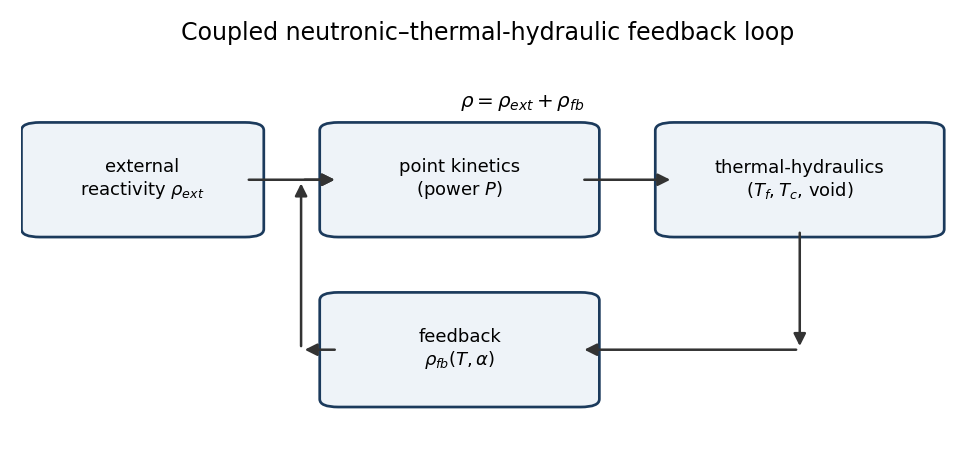
\includegraphics[width=0.95\linewidth]{figures/block.png}
\caption{The coupled neutronic--thermal-hydraulic feedback loop. The sign of the
feedback path $\rho_{fb}(T,\alpha)$ determines stability.}
\label{fig:intro-block}
\end{figure}

The mathematics of the upper path (kinetics) occupies Chapter~\ref{ch:pk}; the
right-hand block (thermal-hydraulics) occupies Chapter~\ref{ch:thermal}; the
feedback path occupies Chapter~\ref{ch:feedback}; and the behaviour of the
\emph{closed} loop---its stability---occupies Part~III.

\section{Two reactors, two fates}

To fix ideas, contrast two reactor philosophies that recur throughout the book.

A \textbf{pressurised-water reactor (PWR)} is deliberately
\emph{under-moderated}. Its lattice is designed so that if the water heats and
expands, or if it boils and forms voids, the moderation of neutrons
\emph{worsens}, the chain reaction weakens, and power falls. Both its moderator
temperature coefficient and its void coefficient are negative. Combined with a
strongly negative Doppler coefficient in the fuel, the PWR is inherently
self-regulating across its operating range: pushing the power up pushes the
temperature up, which pushes the reactivity---and hence the power---back down.

The \textbf{RBMK-1000}, the Soviet design at Chernobyl, was \emph{over-moderated}
by virtue of its large graphite moderator, which is independent of the water
coolant. In the RBMK, the water served mainly as coolant and as a neutron
\emph{absorber}. Boiling the water therefore \emph{removed an absorber} without
removing much moderation, so steam voids \emph{increased} reactivity. Its void
coefficient was strongly positive, especially at low power and with the core
configured as it was on the night of the accident. Pushing the power up boiled
more water, which pushed the reactivity---and the power---further up. The same
nudge that a PWR damps, the RBMK amplified.

\begin{figure}[H]
\centering
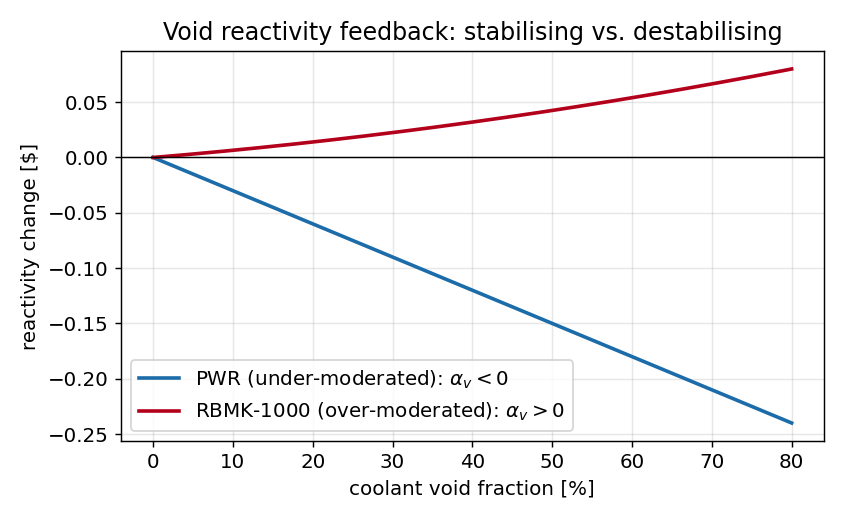
\includegraphics[width=0.78\linewidth]{figures/void.png}
\caption{Schematic void reactivity feedback. In an under-moderated lattice
(PWR) voids reduce reactivity; in an over-moderated lattice (RBMK) voids
increase it. The slope at the operating point is the void coefficient
$\alpha_v$.}
\label{fig:intro-void}
\end{figure}

This single contrast---under-moderated versus over-moderated, negative versus
positive void coefficient---is the physical heart of the Chernobyl story, and we
will return to it repeatedly with increasing precision.

\section{What ``thermal'' stability is not}

It is worth separating thermal stability from several neighbouring concepts that
are sometimes conflated with it.

\emph{Criticality} is a static balance: $\keff=1$, neutron production equals
neutron loss. A reactor can be exactly critical and still be dynamically
unstable. Stability is about what happens to small departures from balance, not
about the balance itself.

\emph{Controllability} is the ability of operators and automatic systems to
drive the reactor to a desired state. A reactor can be controllable yet rely on
that control to remain safe; the ideal is a reactor whose physics keep it safe
even when control fails. Inherent stability reduces the burden on control.

\emph{Thermal-hydraulic stability} in the narrow sense refers to flow and
boiling instabilities (density-wave oscillations, flow excursions) that can
occur even at fixed power. These couple strongly to neutronics in boiling
systems and are part of the broader stability picture treated in
Chapter~\ref{ch:linear}.

\emph{Structural and material stability}---the integrity of fuel, cladding, and
pressure boundary under thermal stress---is the ultimate limit that a power
excursion challenges. Thermal stability theory predicts whether and how fast a
reactor approaches those limits.

\section{Roadmap and how the Chernobyl thread runs through the book}

Each part of this book develops a piece of theory and then points it at
Chernobyl. Part~I gives us the kinetics that explain why the final excursion was
a prompt-critical event measured in seconds. Part~II gives us the feedback
coefficients that explain why the RBMK amplified rather than damped the
disturbance. Part~III gives us the stability criteria that, applied to the
RBMK's operating state that night, predict instability. Part~IV reconstructs the
accident and shows the theory accounting for it in detail. Part~V asks how modern
designs build in the negative feedback that the RBMK lacked, and demonstrates the
dynamics with a small open-source kinetics code.

The recurring lesson is not that the operators were uniquely reckless or that one
component uniquely failed. It is that a reactor with the wrong sign of feedback,
operated into the corner of its envelope where that wrong sign was strongest,
behaved exactly as the equations say such a machine must. Stability is physics;
the accident was the physics asserting itself.


\section*{Exercises}
\addcontentsline{toc}{section}{Exercises}
\begin{enumerate}[leftmargin=*,itemsep=2pt]
\item Explain in one sentence the difference between criticality and stability, and give an example of a reactor state that is critical but unstable.
\item A reactor has a positive void coefficient. Describe qualitatively the sequence of events following a small increase in power, and contrast it with a reactor having a negative void coefficient.
\item Why is it insufficient for a reactor merely to ``settle down'' after a disturbance for it to be called inherently safe? Distinguish stability from controllability.
\item List the three features of reactor physics that make stability non-trivial, and explain which one delayed neutrons mitigate.
\item Using the under-/over-moderated distinction, explain why a PWR and an RBMK respond oppositely to coolant boiling.
\end{enumerate}
